%!TEX root = ../chapter1.tex
%******************************
%	 Results 
%*****************************

\section{scRNAseq of murine CD4$^+$ T cells}
\subsection*{Single-cell RNA sequencing of CD4$^+$ T cells during activation, ageing and across two mouse species}

\begin{wrapfigure}{r}{0.5\textwidth}
\centering    
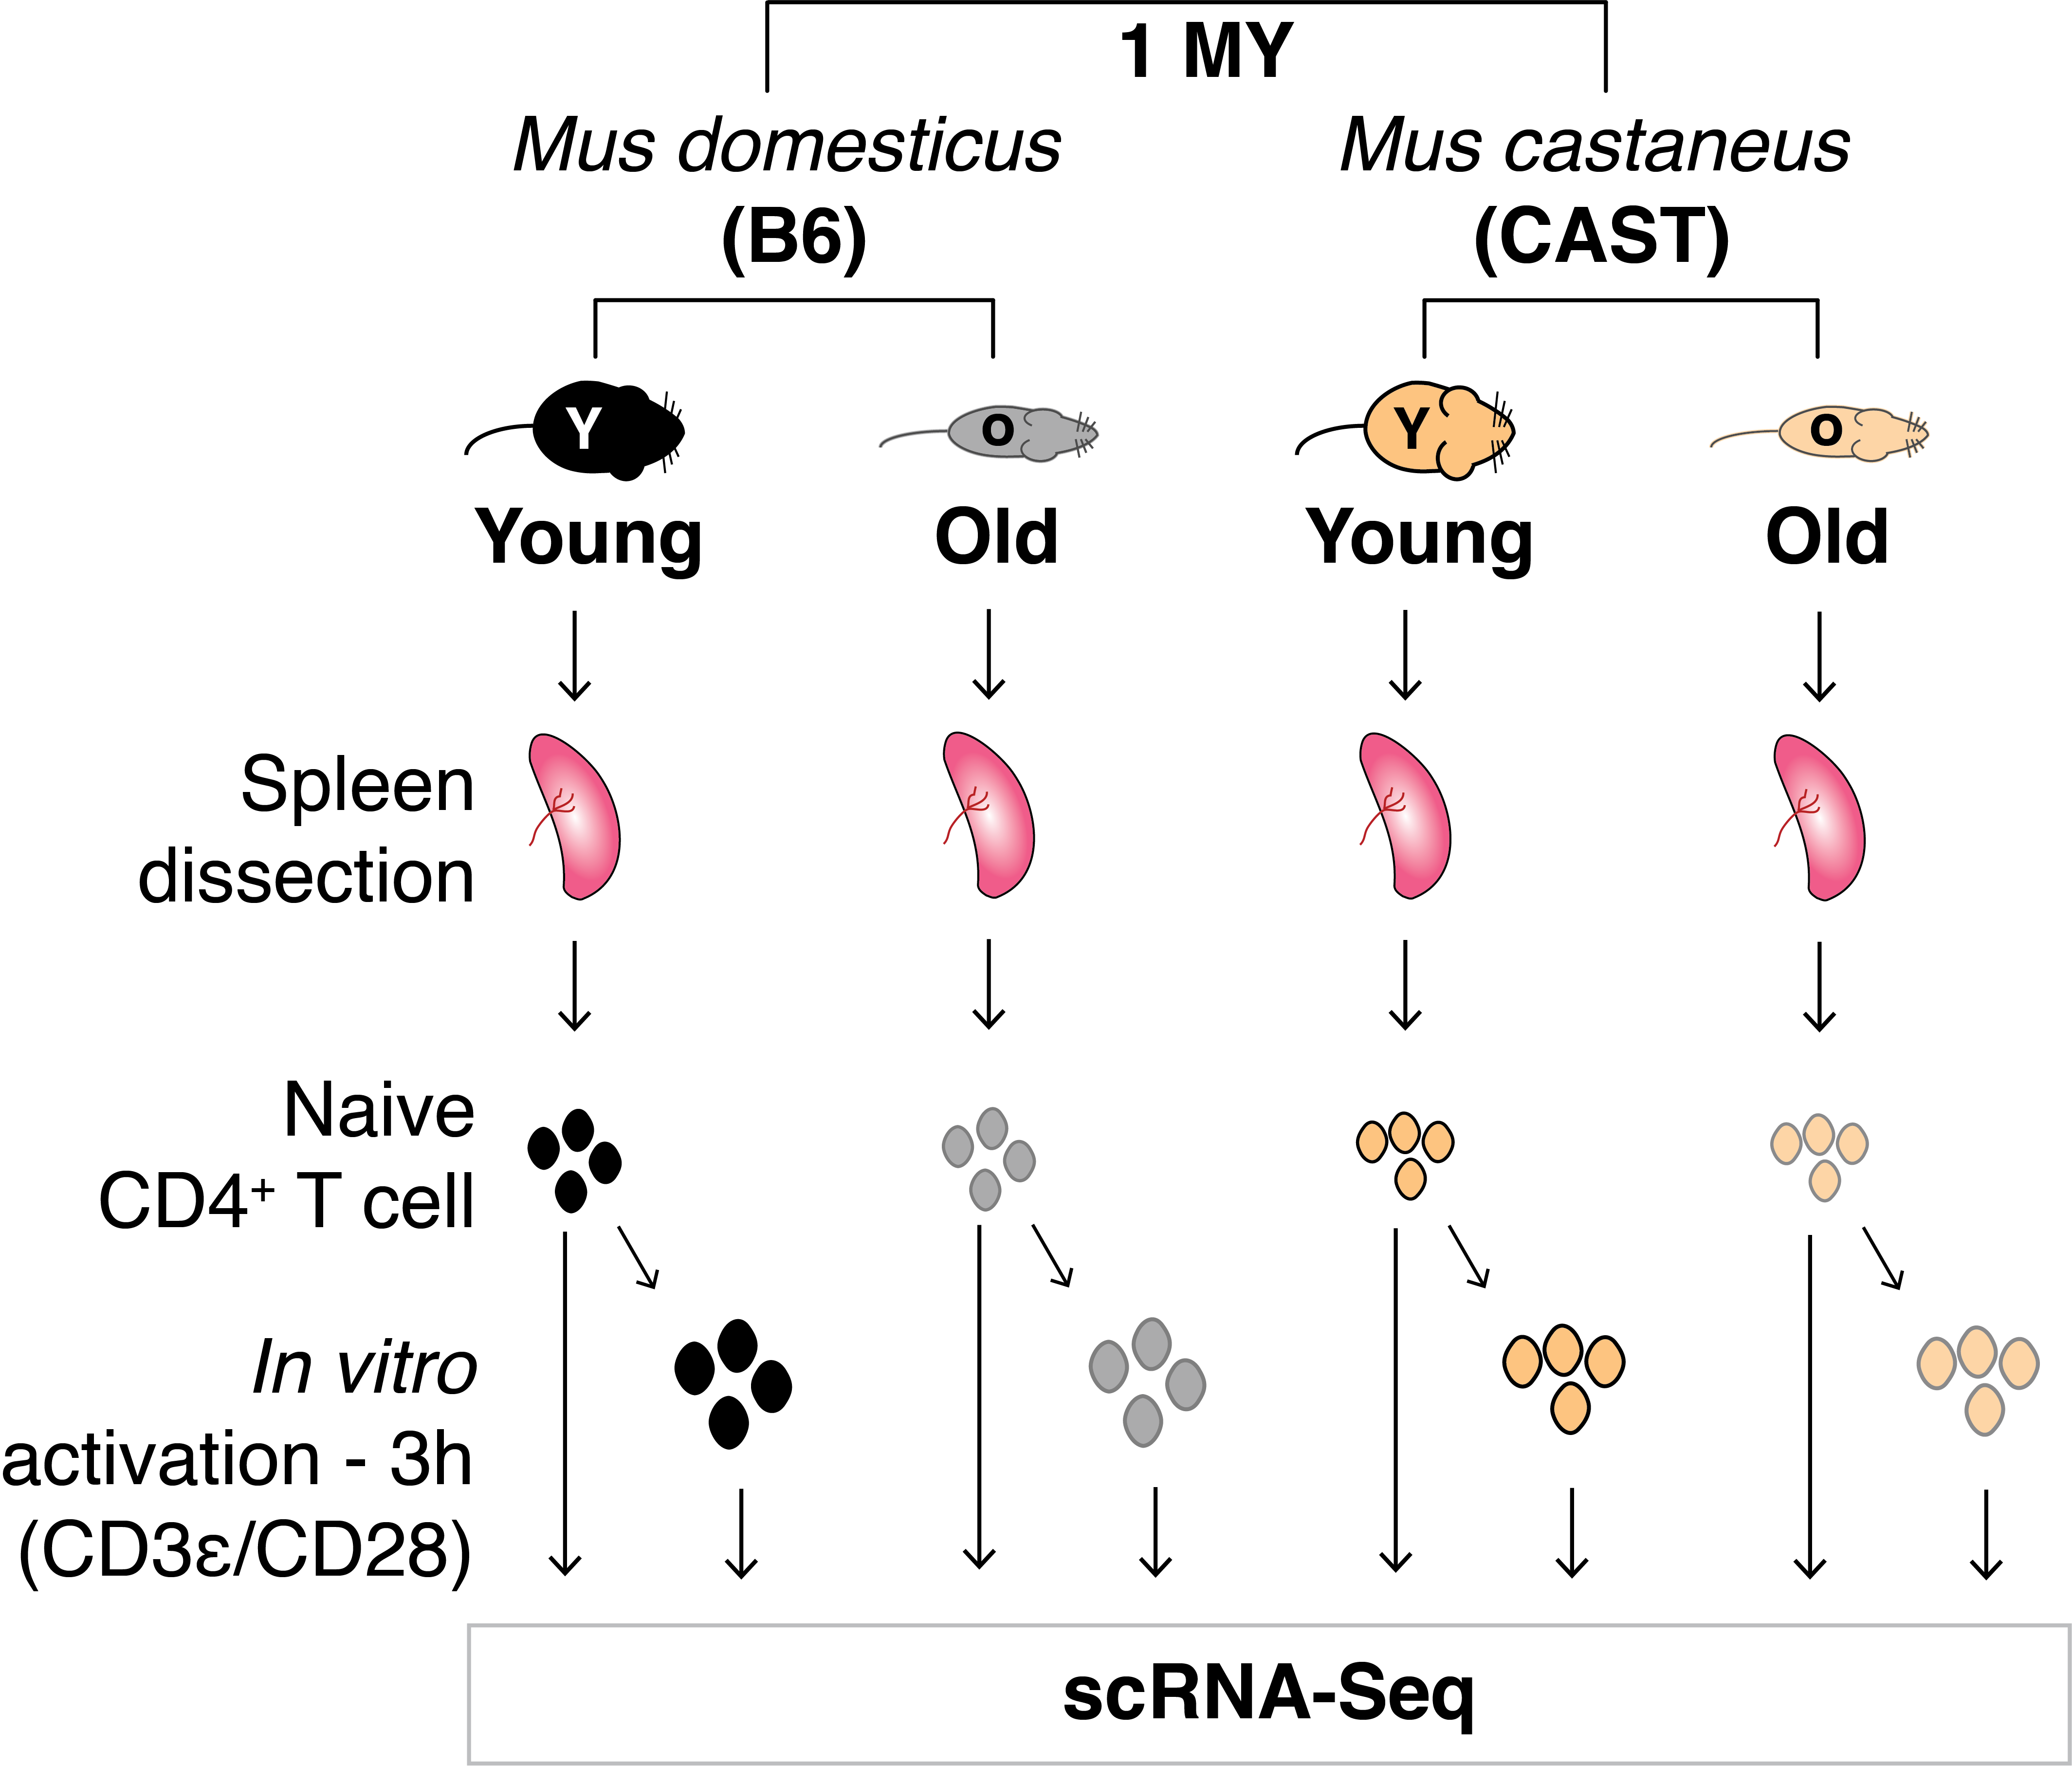
\includegraphics[width=0.48\textwidth]{Fig_1.png}
\caption[scRNAseq of CD4$^+$ T cells from young and old mice.]{\textbf{scRNAseq of unstimulated and activated CD4$^+$ T cells from young and old B6 and CAST animals.} \\
Single cells were isolated from spleens of young (~3 month) and old (~21 month) individuals of two related mouse sub-species (Mus musculus domesticus, B6; Mus musculus castaneus, CAST). Isolated cells were subjected to single-cell mRNA sequencing (scRNAseq) before or after 3 hours of in vitro activation using anti-CD3$\epsilon$/CD28 coated plates.}
\label{fig:chapt1_overview}
\end{wrapfigure}

To assess the conservation of immune activation programmes, we isolated CD4$^+$ T cells from healthy individuals of two inbred mouse sub-species separated by 1 million years of divergence: the reference C57BL/6J, Mus musculus domesticus (B6); CAST/EiJ, Mus musculus castaneus (CAST)). We characterized their gene expression programmes by single-cell RNA-sequencing (scRNAseq) during ageing in young (~3 months) and old (~21 months) individuals of each strain \textbf{(Fig. \ref{fig1:chapt1_overview})}. These two sub-species have similar lifespans \citep{Yuan2011}, and CAST mice showed the hallmarks of normal organismal aging observed in B6 mice \citep{Rodwell2004}. All mice were healthy at the time of experiments. To asses different CD4$^+$ T cell compartments, we assayed cell populations with different levels of purity. First, we isolated all unstimulated CD4$^+$ T cells from spleen of old and young animals. Secondly, we highly purified naive CD4$^+$ T cells and effector memory (EM) CD4$^+$ T cells. For each species/condition, scRNA-seq experiments were performed using cells isolated from two individual mice.

\subsubsection*{Unstimualted CD4$^+$ T cells}

Unstimulated naive CD4$^+$ T cells were purified from dissociated mouse spleens using cell strainers, cell separation media and a MACS CD4$^+$ CD62L$^+$ T Cell Isolation Kit. Purified naive CD4$^+$ T cells were cultured in IMDM medium supplemented with 10\% Fetal Bovine Serum, 1 $\mu$g/mL Penicillin/Streptomicin, and 50 $\mu$M 2-mercaptoethanol. \\

\subsubsection{Naive and effector memory CD4$^+$ T cells}

\begin{wrapfigure}{r}{0.5\textwidth}
\centering    
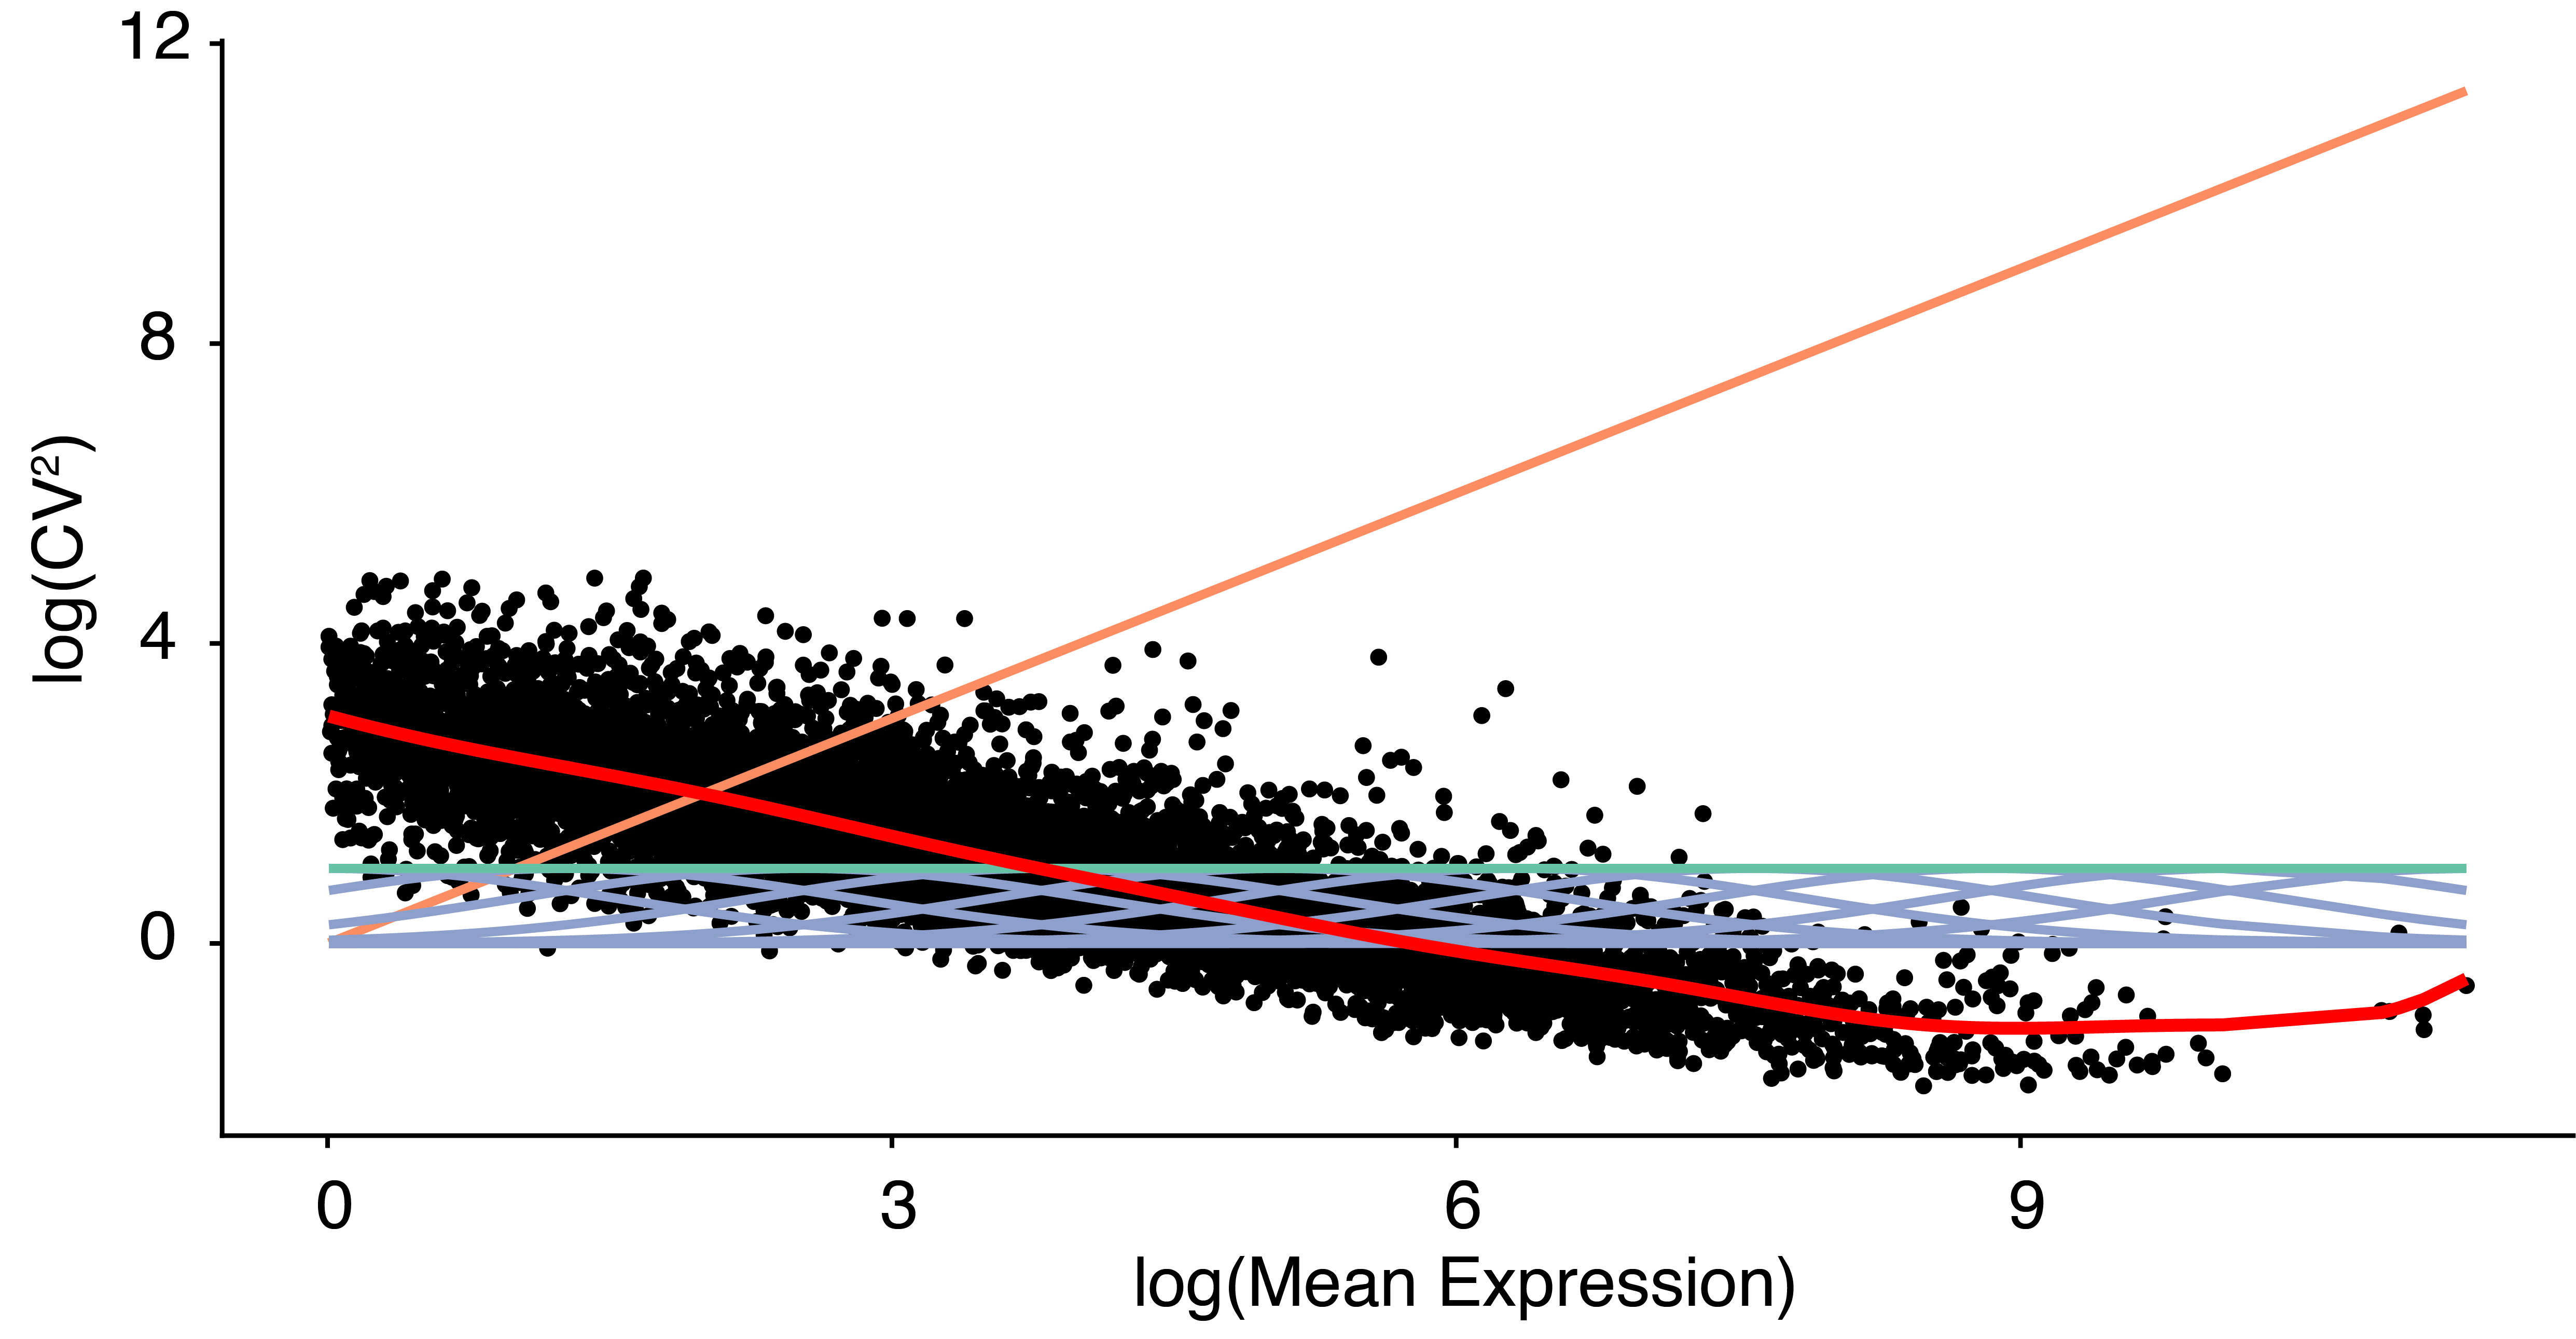
\includegraphics[width=0.48\textwidth]{Fig_2.png}
\caption[FACS of naive and effector mempry CD4$^+$ T cells.]{\textbf{FACS of naive and effector mempry CD4$^+$ T cells.} \\
Gating Strategy: lymphocytes were gated by the use of forward scatter (FSC-A) and side scatter (SSC-A). Cell doublets were excluded according to area and height of forward scatter (FSC-A/FSC-H). Dead cells were removed using viability dye. PD-1$^+$ CD4$^+$ T cells were excluded and PD-1-ve CD4$^+$ T cells were further separated into naive and EM CD4$^+$ T cell subsets according to their CD44 and CD62L expression. Cells with a mature CD24lo Qa2hi phenotype were then gated from naive and EM subsets and CD69+ cells were removed.}
\label{fig1:FACS}
\vspace*{-20mm}
\end{wrapfigure}

Naive and effector memory CD4$^+$ T cells were purified from spleens of both young and old C57/BL6 mice by FACS.  Briefly, spleens were harvested from both young and old animals and single cell suspensions were obtained by meshing through a cell strainer (70 $\mu$m). B cells were depleted from cell suspensions by MACS using CD19 microbeads and red blood cells were lysed with RBC lysis buffer. The enriched cell fraction was then stained with Fixable eFluor 780 viability dye following by Fc receptor blocking with TruStain fcXTM and subsequent staining with a panel of fluorescence-conjugated antibodies against CD4, CD44, CD62L, CD24, Qa2, CD69 and PD-1.  Stained cells were immediately sorted using a 5-laser Aria IIu SORP instrument with the stringent gating strategy described in \textbf{Fig. \ref{fig1:FACS}}. \\
Hereafter, for simplification and clarity, purified unstimulated CD4$^+$ T cells will be named naive, stimulated cells will be named activated.

\subsubsection*{Activation of CD4$^+$ T cells}

Naive cells were seeded into 96-well plates coated for 1h at 37ºC with anti-CD3$\epsilon$ (1 $\mu$g/ml) and anti-CD28 (3 $\mu$g/ml) at a density of 80,000-120,000 cells/ml, and then cultured in a total volume of 100 $\mu$l media that did not contain cytokines or additional antibodies.

\subsubsection*{scRNAseq using the Fluidigm C1 system}

Naive, purified naive and activated CD4+ T cells were immediately collected and loaded on a 5–10$\mu$m Auto Prep Integrated Fluidic Circuit (IFC) to capture single cells using the C1 Single cell Auto Prep System (Fluidigm). All IFCs were visually inspected, and wells with multiple cells or cell debris were marked as low quality. Upon cell capture, reverse transcription and cDNA amplification were performed using the SMARTer PCR cDNA Synthesis Kit and the Advantage 2 PCR Kit. ERCC spike-in RNA (1 $\mu$L diluted at 1:50,000) was added to the C1 lysis mix. All capture sites were included for the RNA-seq library preparation.

\subsubsection*{Read alignment to reference genomes}

Read alignment to reference genomes was performed using \emph{gsnap} with default parameters, while supplying splice-site positions. Samples taken from B6 were mapped against the mouse reference GRCm38. CAST samples were aligned against the \emph{Mus musculus castaneus de novo} genome assembly [ftp://ftp-mouse.sanger.ac.uk/REL-1509-Assembly/], which was used under an advance access agreement [ftp://ftp-mouse.sanger.ac.uk/REL-1509-Assembly/README]. Gene annotation for B6 was taken from the GRCm38 reference; gene annotation for CAST was taken from the newly constructed \emph{Mus musculus castaneus} assembly [http://hgwdev.cse.ucsc.edu/$\sim$ifiddes/mouse\_{}genomes\_{}data/, version 0.2]. Additionally, since mitochondrial genes and certain immune genes (e.g., CD28) are absent from the most recent \emph{Mus musculus castaneus} annotation, and since high mitochondrial gene expression is a well-established signature of low-quality single-cell transcriptome profiles \citep{Ilicic2016}, we also mapped CAST reads against GRCm38 and used the B6 annotation solely for these genes. Gene expression counts were obtained using HTSeq with default options. Only genes with orthologs in both species were considered for downstream analysis. 

\subsubsection*{Computational quality control and filtering}

We visually inspected the vast majority of cell-capture sites in each C1 small-integrated fluidic circuit using 40x magnification lensing to ensure precise capture of single cells \textbf{(Fig. \ref{fig1:QC}A and B)}. Low-quality cells were computationally filtered using the following quality control criteria, developed by previous single-cell RNA-sequencing studies \citep{Brennecke2015, Buettner2015, Scialdone2015, Vallejos2015}:\\
The percentage of reads mapping to annotated genomic regions was compared to the percentage of reads mapping to ERCC spike-ins. Cells with low genomic read (< 20\%) and/or high ERCC read (> 50\%) numbers were excluded \textbf{(Fig. \ref{fig1:QC}C)}. Additionally, cells with few mapped reads (< 1,000,000) or in which > 3000 or < 1250 genes were detected were removed \textbf{(Fig. \ref{fig1:QC}D and E)}. Next, cells with more than 10\% or less than 0.5\% of mitochondrial reads were excluded \textbf{(\ref{fig1:QC}F)}. Further, known markers of lymphocytes were used to filter cells - CD19$^+$/H2-Aa$^+$ B cells as well as CD8+ T cells were removed \textbf{(Fig. \ref{fig1:QC}H)}. Finally, in stimulated conditions, non-activated T cells were computationally removed \textbf{(Fig. \ref{fig1:QC}I)}.


\begin{figure}[!hb]
\centering
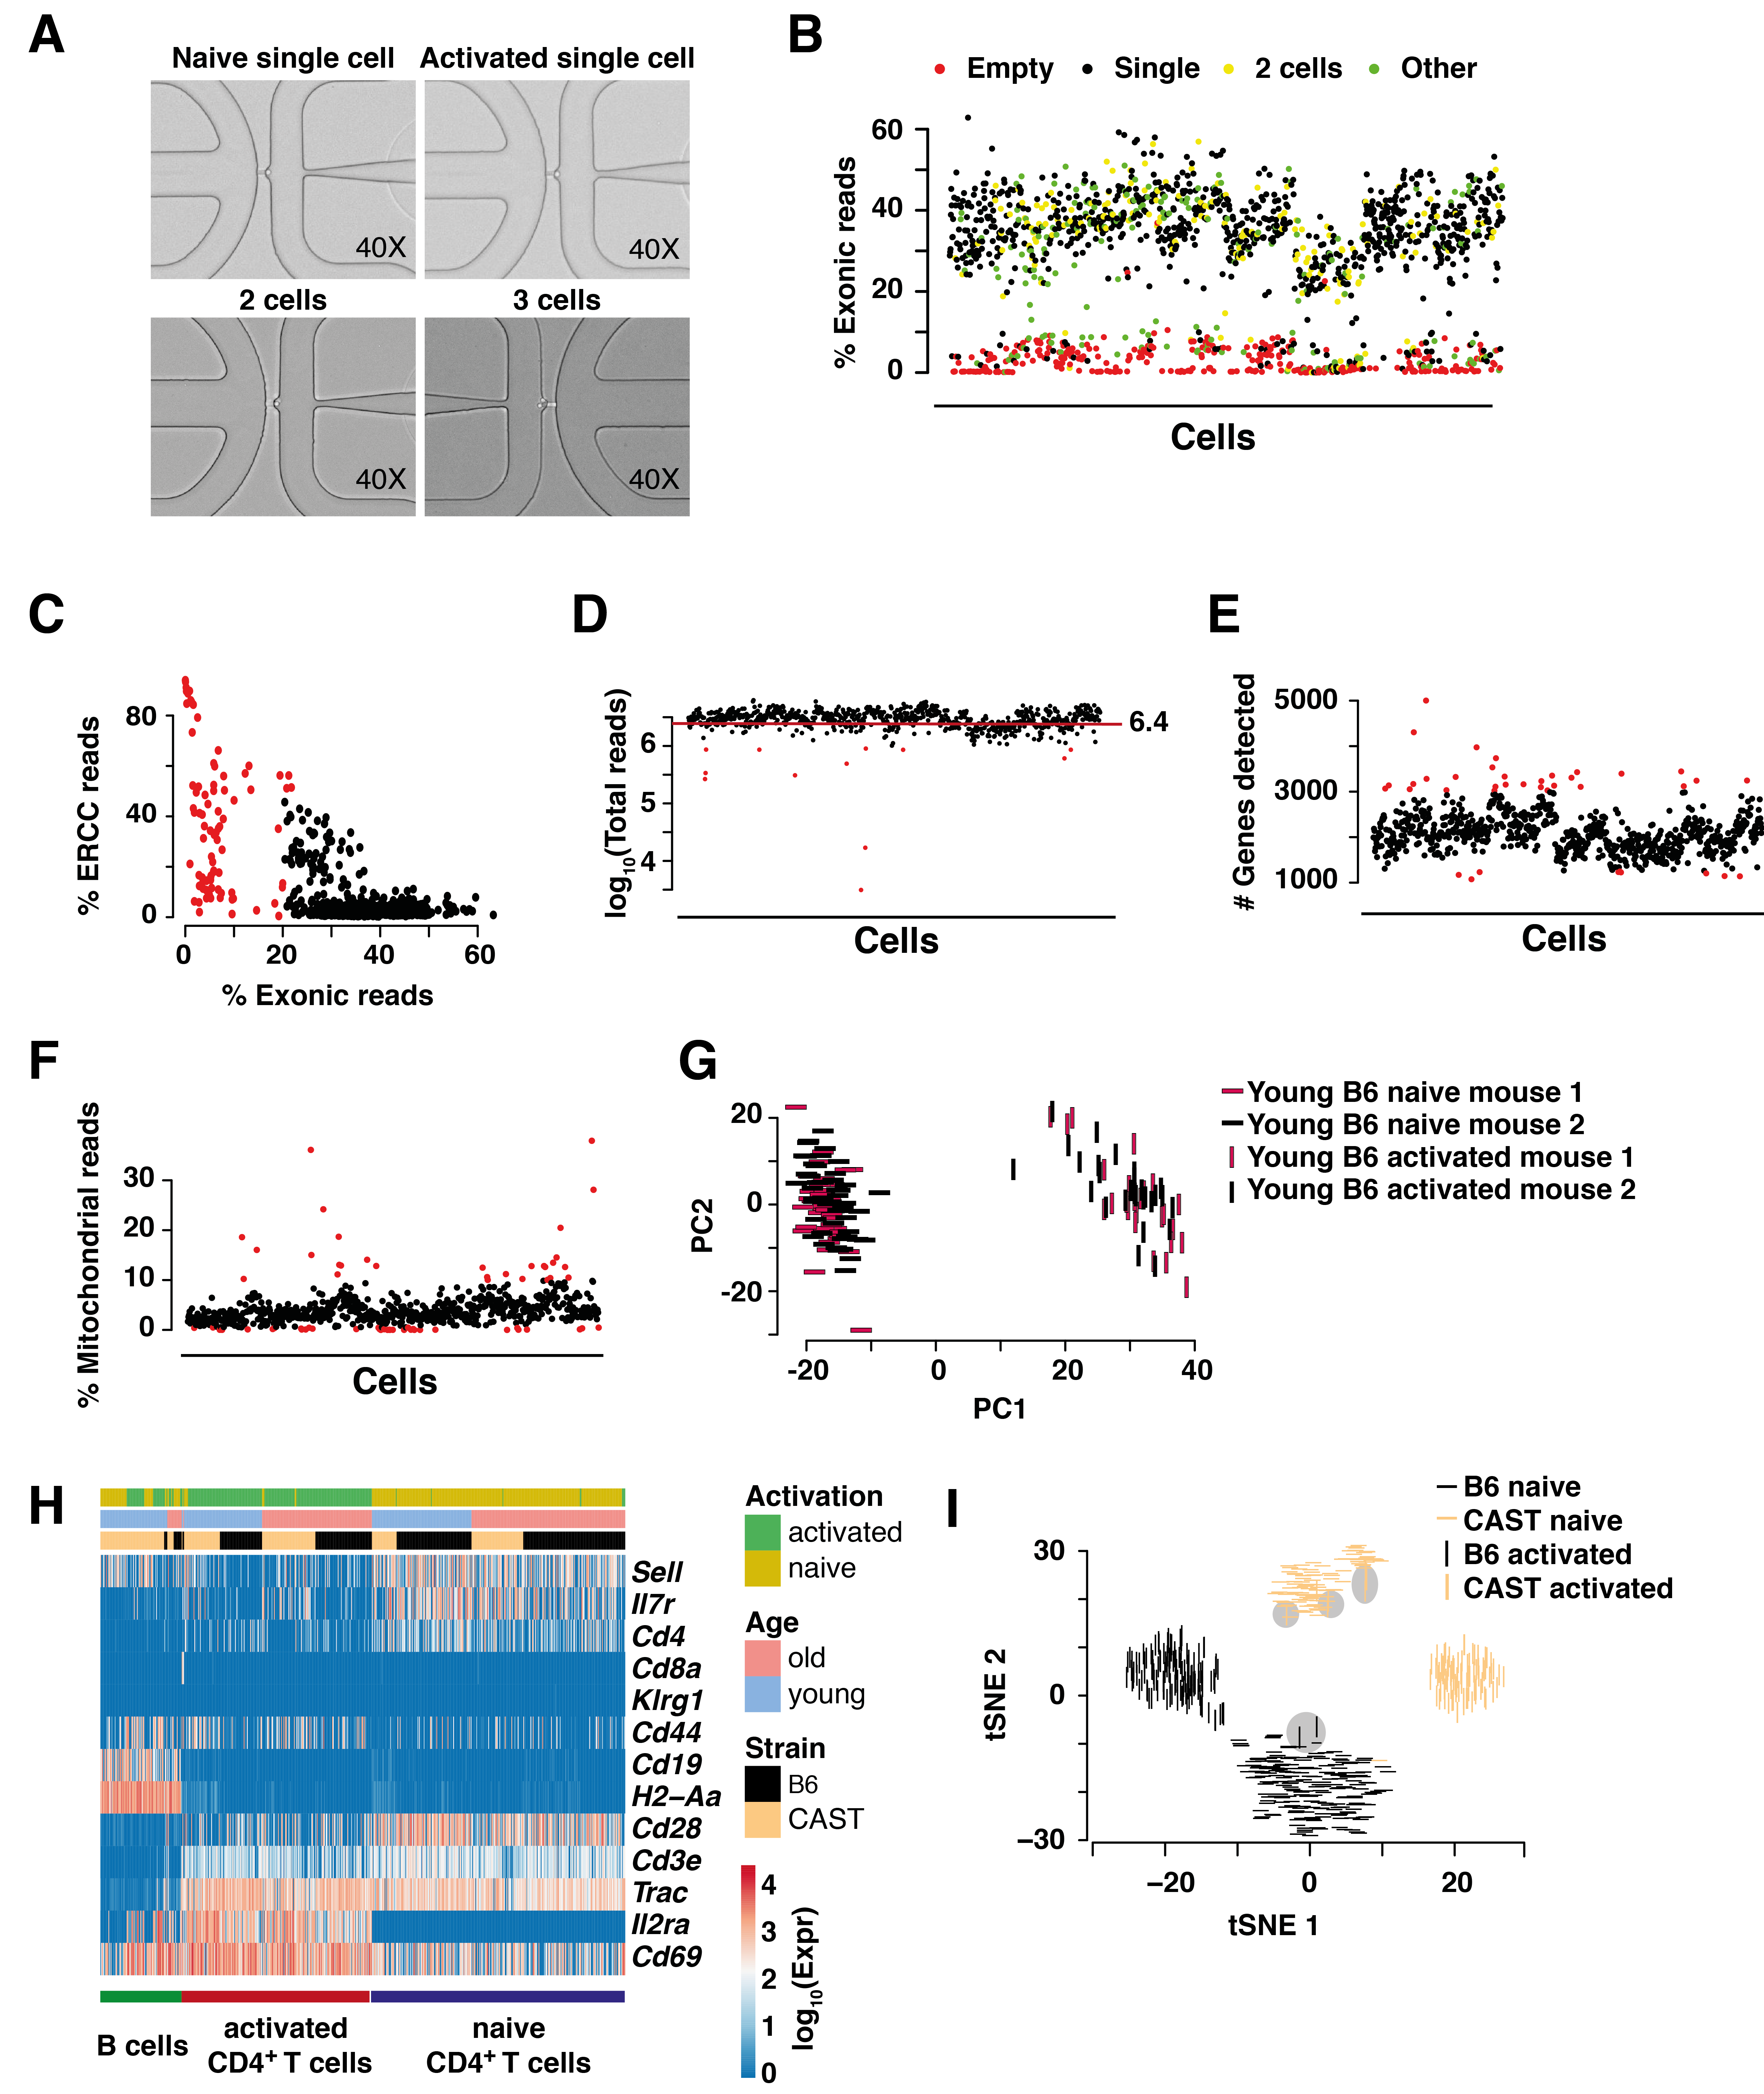
\includegraphics[width=0.9\textwidth,trim={0 4cm 0 0},clip]{Fig_3.png}
\caption[Quality control of isolated CD4$^+$ T cells]{\textbf{Quality control of isolated CD4$^+$ T cells (Full legend on next page).}}
\label{fig1:QC}
\end{figure}

\newpage

\captionsetup[figure]{list=no}
\addtocounter{figure}{-1}   
\captionof{figure}{\textbf{Quality control of isolated CD4$^+$ T cells (continued).}\\
\textbf{(A)} Visual inspection of captured cells at 40x magnification in Integrated Fluidic Circuit (C1, Fluidigm) allows manual removal of empty capture sites, and capture sites holding multiple cells or debris \textbf{(B)} Percentage of reads mapping to exonic regions displayed for naive and activated CD4$^+$ T cells. Black dots: single cells; yellow dots: 2 cells, red dots: empty wells, green dots: debris, multiple cells, etc.; \textbf{(C)} Removal of cells with less than 20\% of mapped exonic reads and more than 50\% of ERCC spike-in reads (red dots);
\textbf{(D)} Cells with less than 1 million mapped reads were excluded from downstream analysis (red dots);  \textbf{(E)} Cells with more than 3000 or less than 1250 genes detected were excluded in the analysis (red dots); \textbf{(F)} Cells with more than 10\% or less than 0.5\% of mitochondrial reads were excluded for downstream analysis (red dots); \textbf{(G)} Naive and activated cells isolated from young B6 animals (replicates) were coloured batch-specifically. 4 batches from 2 mice: naive and activated from mouse 1 (white bars), naive and activated from mouse 2 (black bars). Naive condition is represented in horizontal bars and activated condition in vertical bars; \textbf{(H)} Data set was filtered for immune markers to exclude B cell and CD8$^+$ T cell contamination. Cells in columns were labelled based on their activation state (naive in beige, activated in green), their age (old in red, young in blue), and the strain of the animals (B6 in black, CAST in yellow); \textbf{(I)} Unbiased tSNE clustering allowed the removal of not fully activated cells (indicated in grey circles). Cells were labelled based on their activation state (naive: horizontal bar, activated: vertical bar) and the strain of the animals (B6 in black, CAST in yellow).
.}
\captionsetup[figure]{list=yes}

\subsubsection*{Characterization of isolated CD4$^+$ T cells}

In contrast to haematopoeitic cells \citep{Kowalczyk2015}, even when activated, virtually all CD4$^+$ T cells are in G1 phase of cell cycle as expected \textbf{(Fig. \ref{fig1:characterization}A)}. Aged CD4$^+$ T cells showed no clonal expansions \textbf{(Fig. \ref{fig1:characterization}B)} or difference in cell size \textbf{(Fig. \ref{fig1:characterization}C)} that could impact analysis of gene expression variability \citep{Stubbington2015}. Using flow cytometry analysis, we confirmed that 96.4\% of the isolated CD4+ T cells were naive in young B6 \textbf{(Fig. \ref{fig1:characterization}D)}. Naive CD4+ T cells formed a single, high-purity population in young animals. Old animals had a small population of CD4$^+$ T cells with slightly elevated CD44 levels, reduced CD62L expression, and attenuated activation dynamics \textbf{(Fig. \ref{fig1:characterization}E-G)}. Upon T cell receptor (TCR) activation in the presence of particular cytokines, naive CD4$^+$ T cells can differentiate into several lineages of functionally different T helper cells (mainly Th1, Th2, Th17, Treg, Tfh) \citep{Stubbington2015, Zhu2010}. In our data we do not detect any early differentiation in naive and activated CD4$^+$ T cell subsets. In accordance with the literature we found \textit{Gata3} but not Th2 cytokines expressed in the majority of cells  \citep{Ho2009}. Interestingly, the Th1-related genes \textit{Tbx21} and \textit{Ifng} were up-regulated, in an uncoordinated manner, in a small population of activated CD4$^+$ T cells of old animals. This is consistent with a known Th1 bias in CD4$^+$ T cell responses in old mice \citep{Zhang2014} and humans \citep{Sakata-Kaneko2000} \textbf{(Fig. \ref{fig1:characterization}H)}. Furthermore, we did not detect any difference in TCR components/signaling and importantly detected no signs of T cell exhaustion \citep{Wherry2011}, especially in cells isolated from old animals \textbf{(Fig. \ref{fig1:characterization}I)}. We also ruled out species-specific differences in commitment towards T helper cell lineages \textbf{(Fig. \ref{fig1:characterization}J-K)}. \\

\begin{figure}[!hb]
\centering
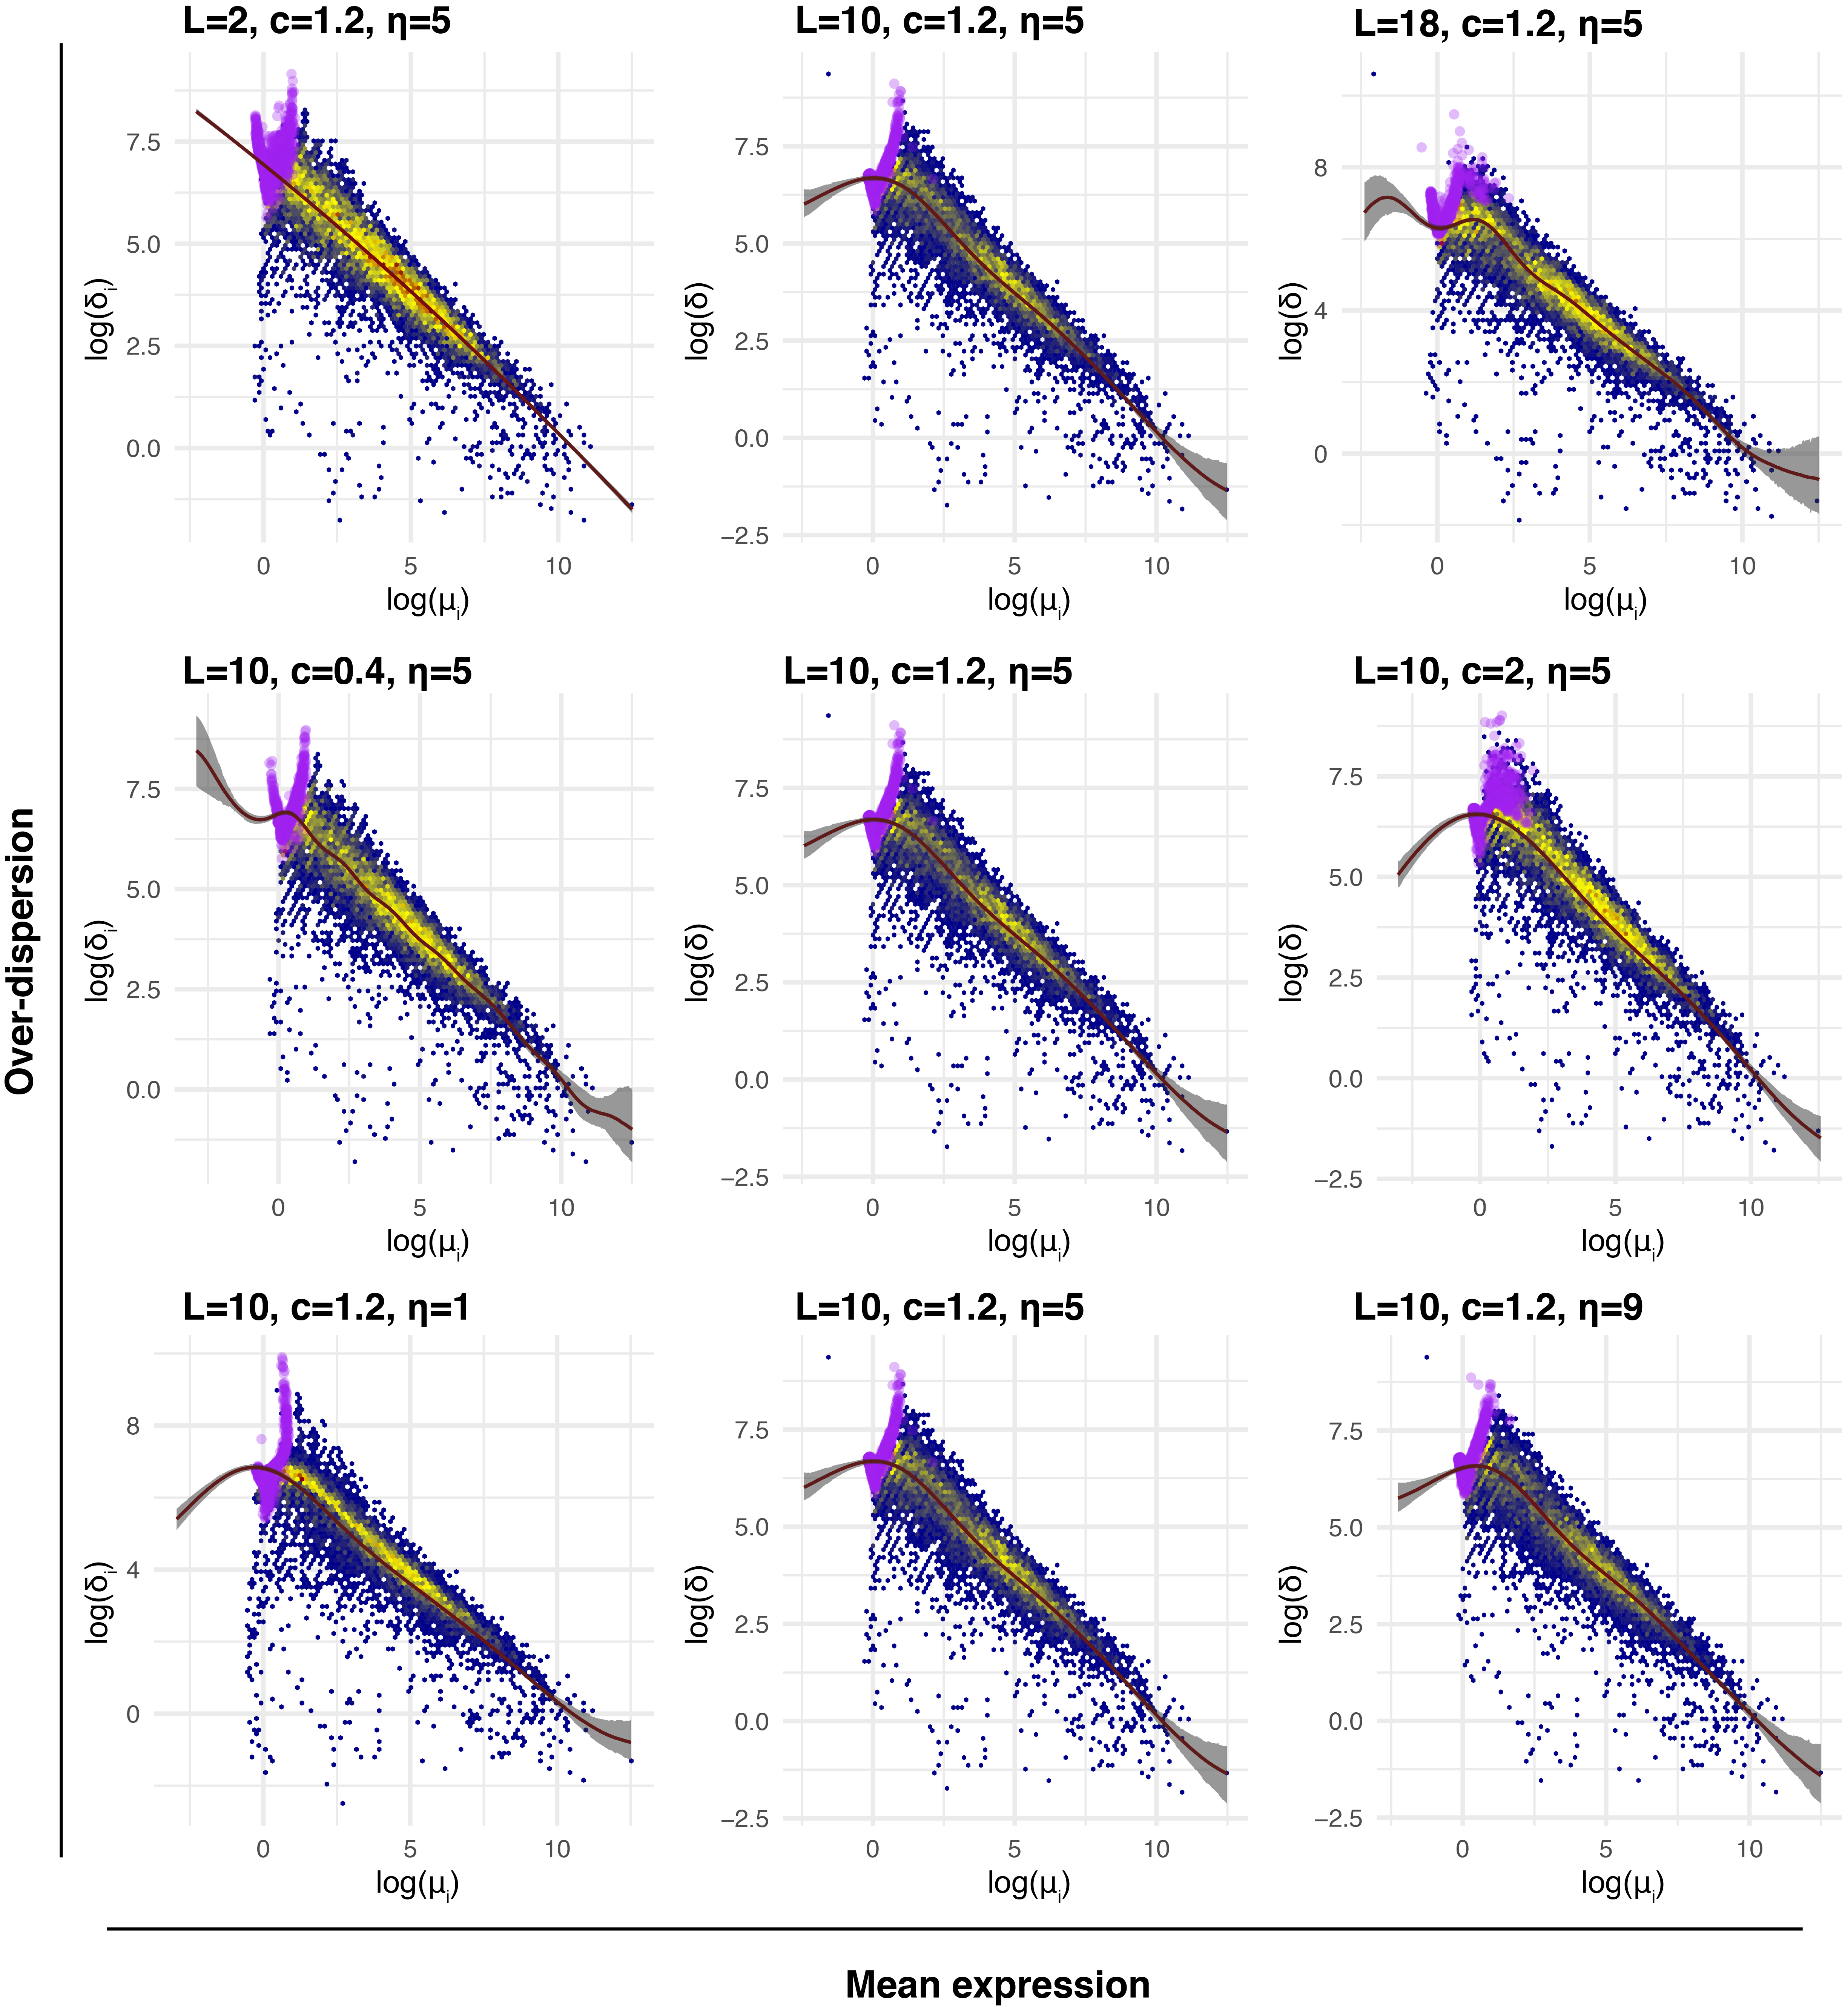
\includegraphics[width=0.8\textwidth]{Fig_4.png}
\caption[Characterization of isolated CD4$^+$ T cells]{\textbf{Characterization of isolated CD4$^+$ T cells (Full legend on next page).}}
\label{fig1:characterization}
\end{figure}

\newpage
\captionsetup[figure]{list=no}
\addtocounter{figure}{-1}   
\captionof{figure}{\textbf{Characterization of isolated CD4$^+$ T cells (continued).}\\
\textbf{(A)} Cyclone \citep{Scialdone2015} was used to classify individual naive and activated CD4+ T cells into the cell cycle phases G1, G2/M and S; \textbf{(B)} TraCeR \citep{Stubbington2015} constructed T cell receptor sequences from scRNA-seq data to analyze clonal diversity in naive and activated CD4$^+$ T cells; \textbf{(C)} Cell sizes were estimated for naive and activated CD4$^+$ T cells in young and old B6 animals measured by forward scatter (FSC-A) using flow cytometry; \textbf{(D)-(E)} CD4$^+$ T cells were purified from spleens of young (D) and old (E) B6 animals and stained with antibodies against CD4, CD62L, CD44, CD69, IL2R$\alpha$ (CD25), CD127, and KLRG1 as well as viability dye. FACS plots shown are gated on single live cells (top left panel) and single live CD4$^+$ T cells (other panels), and percentages shown relate to total of gated cells; \textbf{(F)-(G)} Naive CD4$^+$ T cells were purified from spleens of five young (F) or two aged (G) B6 mice, and were left naive or were activated with plate-bound antibody against CD3$\epsilon$ and CD28 for 3 hours. Cells were stained with antibodies against CD4, CD69, and viability dye. Representative histograms are shown and were gated on single live CD4$^+$ T cells: naive (red) and activated (blue) cells are shown; \textbf{(H)} Characterization of possible differentiation processes leading to T helper 1 (Th1), T helper 2 (Th2), T helper 17 (Th17), regulatory T (Treg) and follicular helper T (Tfh) cell lineages. For each lineage the major regulatory transcription factor (upper row) and an effector cytokine (lower row) is shown. Statistical differential expression testing was performed between activated and naive cells from young B6 animals (left panel) and between activated and naive cells from old B6 animals (right panel). Upward arrow: up-regulation of expression (log2FC > 2, FDR < 0.05) after activation, Downward arrow: down-regulation of expression (log2FC > 2, FDR < 0.05) after activation; \textbf{(I)} Heatmap showing T cell exhaustion (Pdcd1, Lag3, Havcr2, Ctla4) and TCR activation markers (Cd5). Statistical differential expression testing was performed in naive cells between young and old B6 animals (left panel) and in activated cells between young and old B6 animals (right panel). Upward arrow: up-regulation of expression (log2FC > 2, FDR < 0.05) during aging; \textbf{(J)} Th1 lineage marker (Tbx21, Ifng) expression was compared between B6 and CAST in following conditions: naive cells from young animals (upper left panel), naive cells from old animals (lower left panel), activated cells from young animals (upper right panel), activated cells from old animals (lower right panel). \#: statistically significant differential expression (log2FC > 2, FDR < 0.05); \textbf{(K)} Th2 lineage marker (Gata3, Il4) expression was compared between B6 and CAST in following conditions: naive cells from young animals (upper left panel), naive cells from old animals (lower left panel), activated cells from young animals (upper right panel), activated cells from old animals (lower right panel).
\\}
\captionsetup[figure]{list=yes}

After the above analyses and the experimental characterization, a total of 1514 high-quality CD4$^+$ T cell transcriptomes were analysed across all conditions and species. An overview of all high-quality transcriptomes can be seen in \textbf{Fig. \ref{fig1:all_cells}}. We detect that unstimulated and stimulated cells group together \textbf{(Fig. \ref{fig1:all_cells}A)} while separation is also noticeable between strains \textbf{(Fig. \ref{fig1:all_cells}B)} and experimental methods \textbf{(Fig. \ref{fig1:all_cells}C)}. As discussed below, cells from young and old animals do not separate when visualizing the cells in form of a t-distributed stochastic neighbour embedding (tSNE, \textbf{Fig. \ref{fig1:all_cells}C}). 

\newpage

\begin{figure}[!hb]
\centering
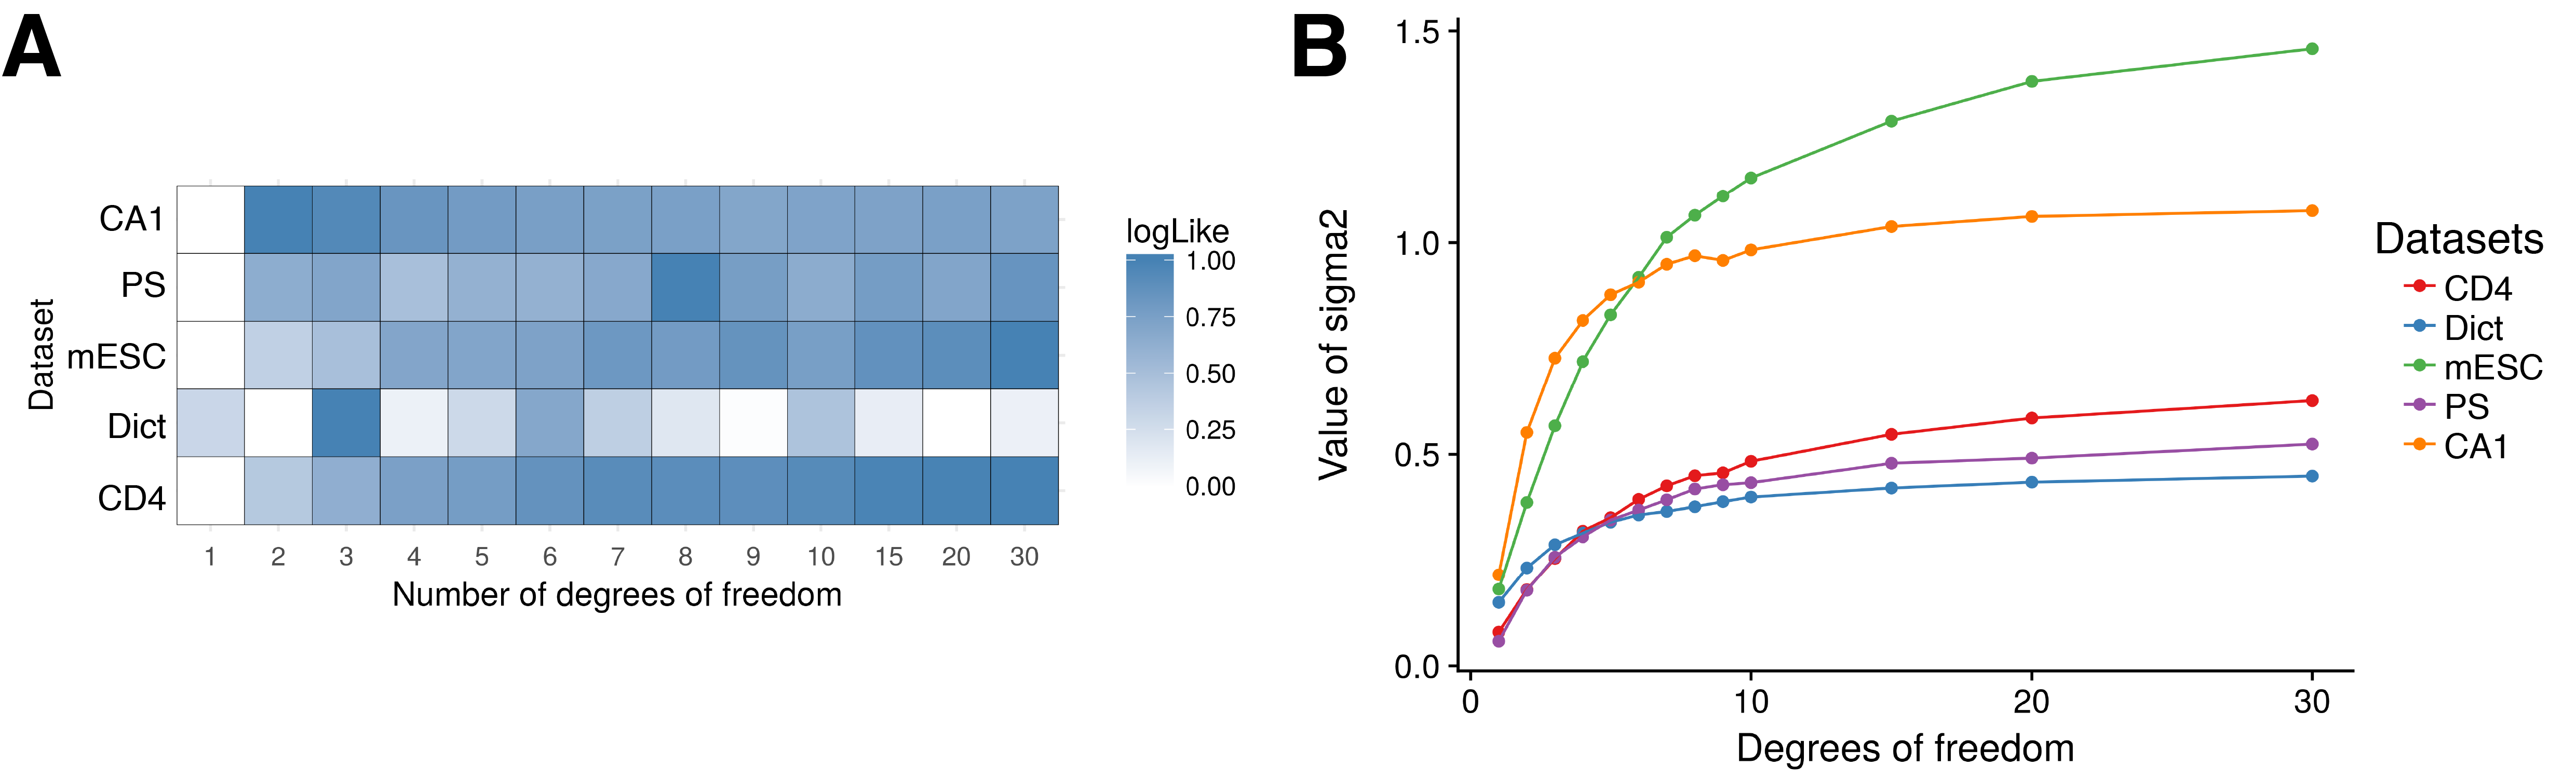
\includegraphics[width=0.8\textwidth]{Fig_5.png}
\caption[Visualization of all isolated CD4$^+$ T cells]{\textbf{Visualization of all isolated CD4$^+$ T cells.}\\
tSNE dimensionality reduction of 1514 CD4$^+$ T cells isolated from young and old mice of two related strains. Cells were labelled based on \textbf{(A)} their activation state, \textbf{(B)} the mouse strain, \textbf{(C)} experimental isolation approach and \textbf{(D)} age.}
\label{fig1:all_cells}
\end{figure}

\section{Species-specific gene expression in naive CD4$^+$ T cells}
\subsection*{Single-cell RNA-seq reveals species-specific gene expression in naive CD4+ T cells}

To fully characterize the variation observed in \textbf{Fig. \ref{fig1:all_cells}}, we dissected differences in gene expression between the two different mouse strains for naive CD4$^+$ T cells. Similar for \textbf{Fig. \ref{fig1:all_cells}}, we found that naive CD4+ T cells cluster by species when only profiling naive CD4$^+$ T cells \textbf{(Fig. \ref{fig1:species_specific})}.

\newpage

\begin{figure}[!hb]
\centering
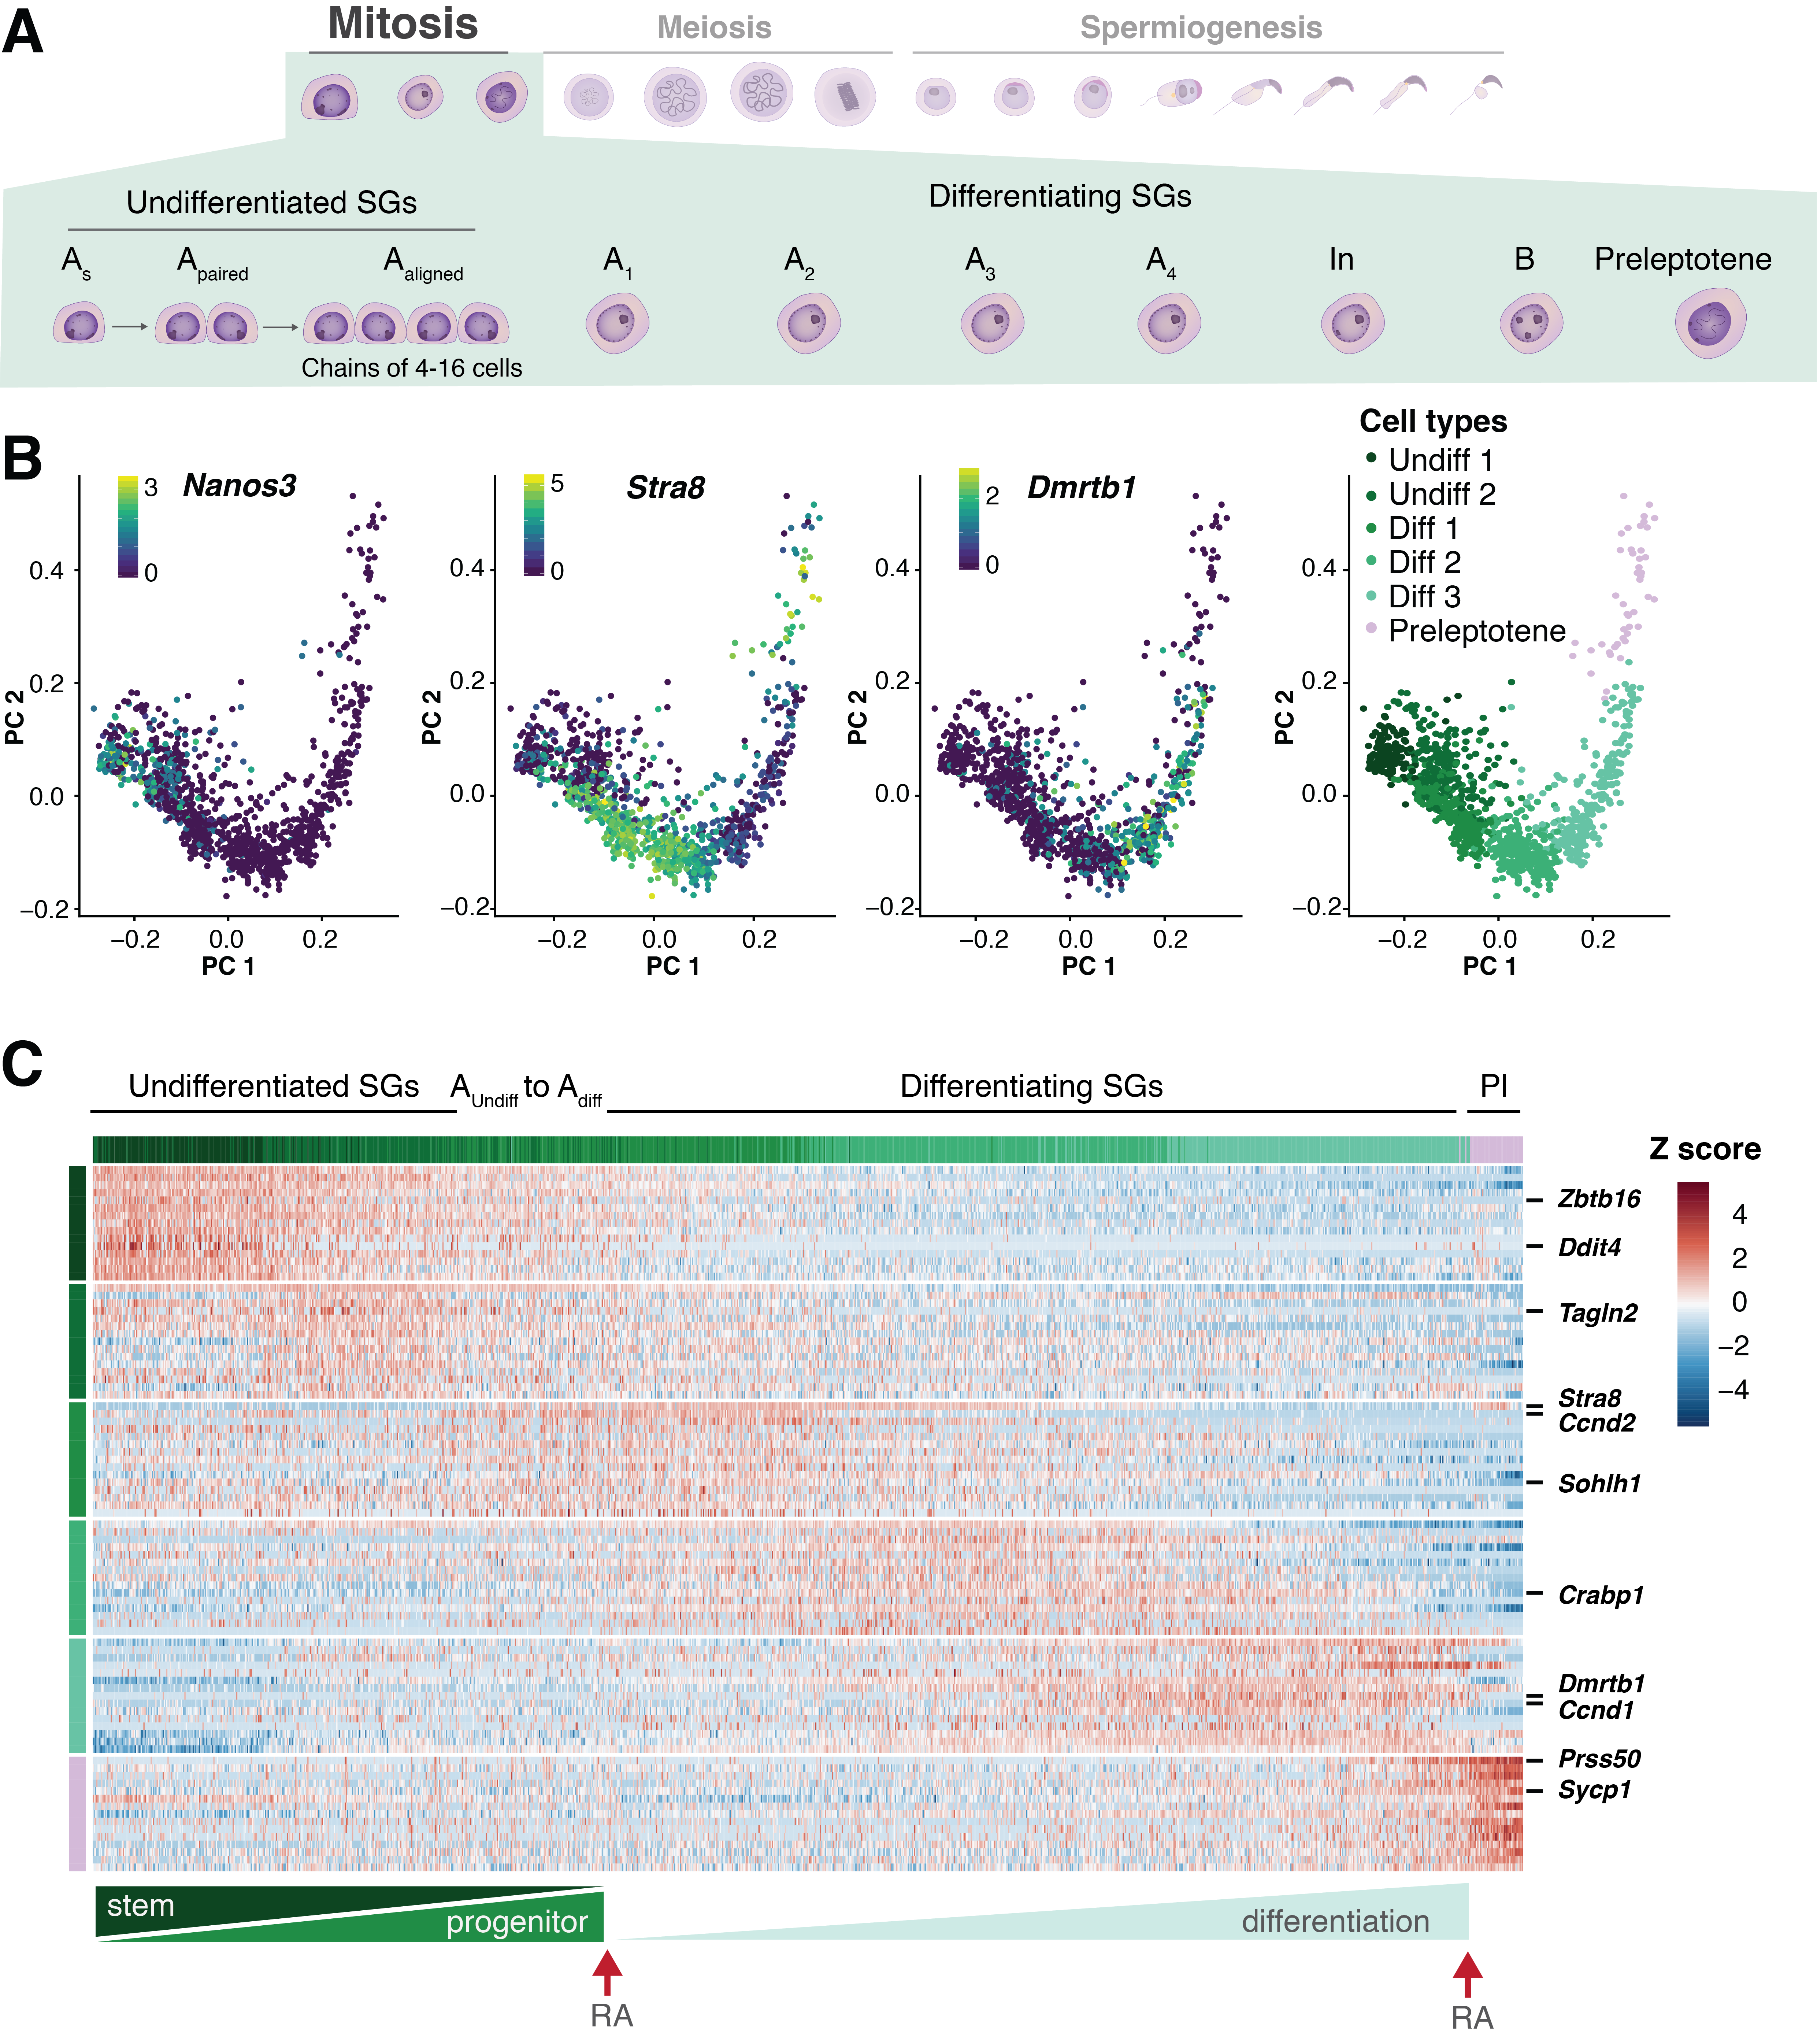
\includegraphics[width=\textwidth]{Fig_6.png}
\caption[Visualization of all isolated CD4$^+$ T cells]{\textbf{Visualization of all isolated CD4$^+$ T cells.}\\
tSNE dimensionality reduction of 1514 CD4$^+$ T cells isolated from young and old mice of two related strains. Cells were labelled based on \textbf{(A)} their activation state, \textbf{(B)} the mouse strain, \textbf{(C)} experimental isolation approach and \textbf{(D)} age.}
\label{fig1:species_specific}
\end{figure}

We used BASiCS \citep{Vallejos2016} to identify differences between mouse species in (a) levels of gene expression and (b) variability of gene expression -- the latter of which is only possible to evaluate genome-wide using single-cell RNA-seq. We observed that 15\% of expressed genes were transcribed differentially between the two mouse species’ CD4$^+$ T cells. 

To rule out the possibility that this clustering is driven by potential artifacts in the new Mus musculus Castaneus genome assembly, we also mapped reads from young CAST samples to the GRCm38 genome. All results presented were unaltered when the GRCm38 reference and annotation was used for both (Fig. S3).

To estimate which differentially expressed genes may arise due to errors in the new CAST genome assembly, we performed the same differential expression analysis on CAST samples by mapping these experiments onto both GRCm38 and CAST. Roughly 5\% of all tested genes are detected as differentially expressed even though the samples being compared are identical and only mapped to different genomes (Fig. S3C). Comparing this set of genes to the set of species-specific genes, we find that they make up 10% of differentially expressed genes between the two species, as expected (36). We performed a similar analysis for B6 samples. This approach allowed us to remove from our analyses the genes showing differences in expression, which may be driven by the quality of the reference genome. 



These differentially transcribed genes were not the result of errors in genome assembly or read mapping, which we estimated may cause inaccuracies in up to only 3\% of transcribed genes (Fig. S3A and S3B). These genes were removed from further analyses. Remaining species-specific genes were not enriched for any functional ontology in either B6 or CAST (Fig. S3C and S3D). 

\begin{figure}[!hb]
\centering
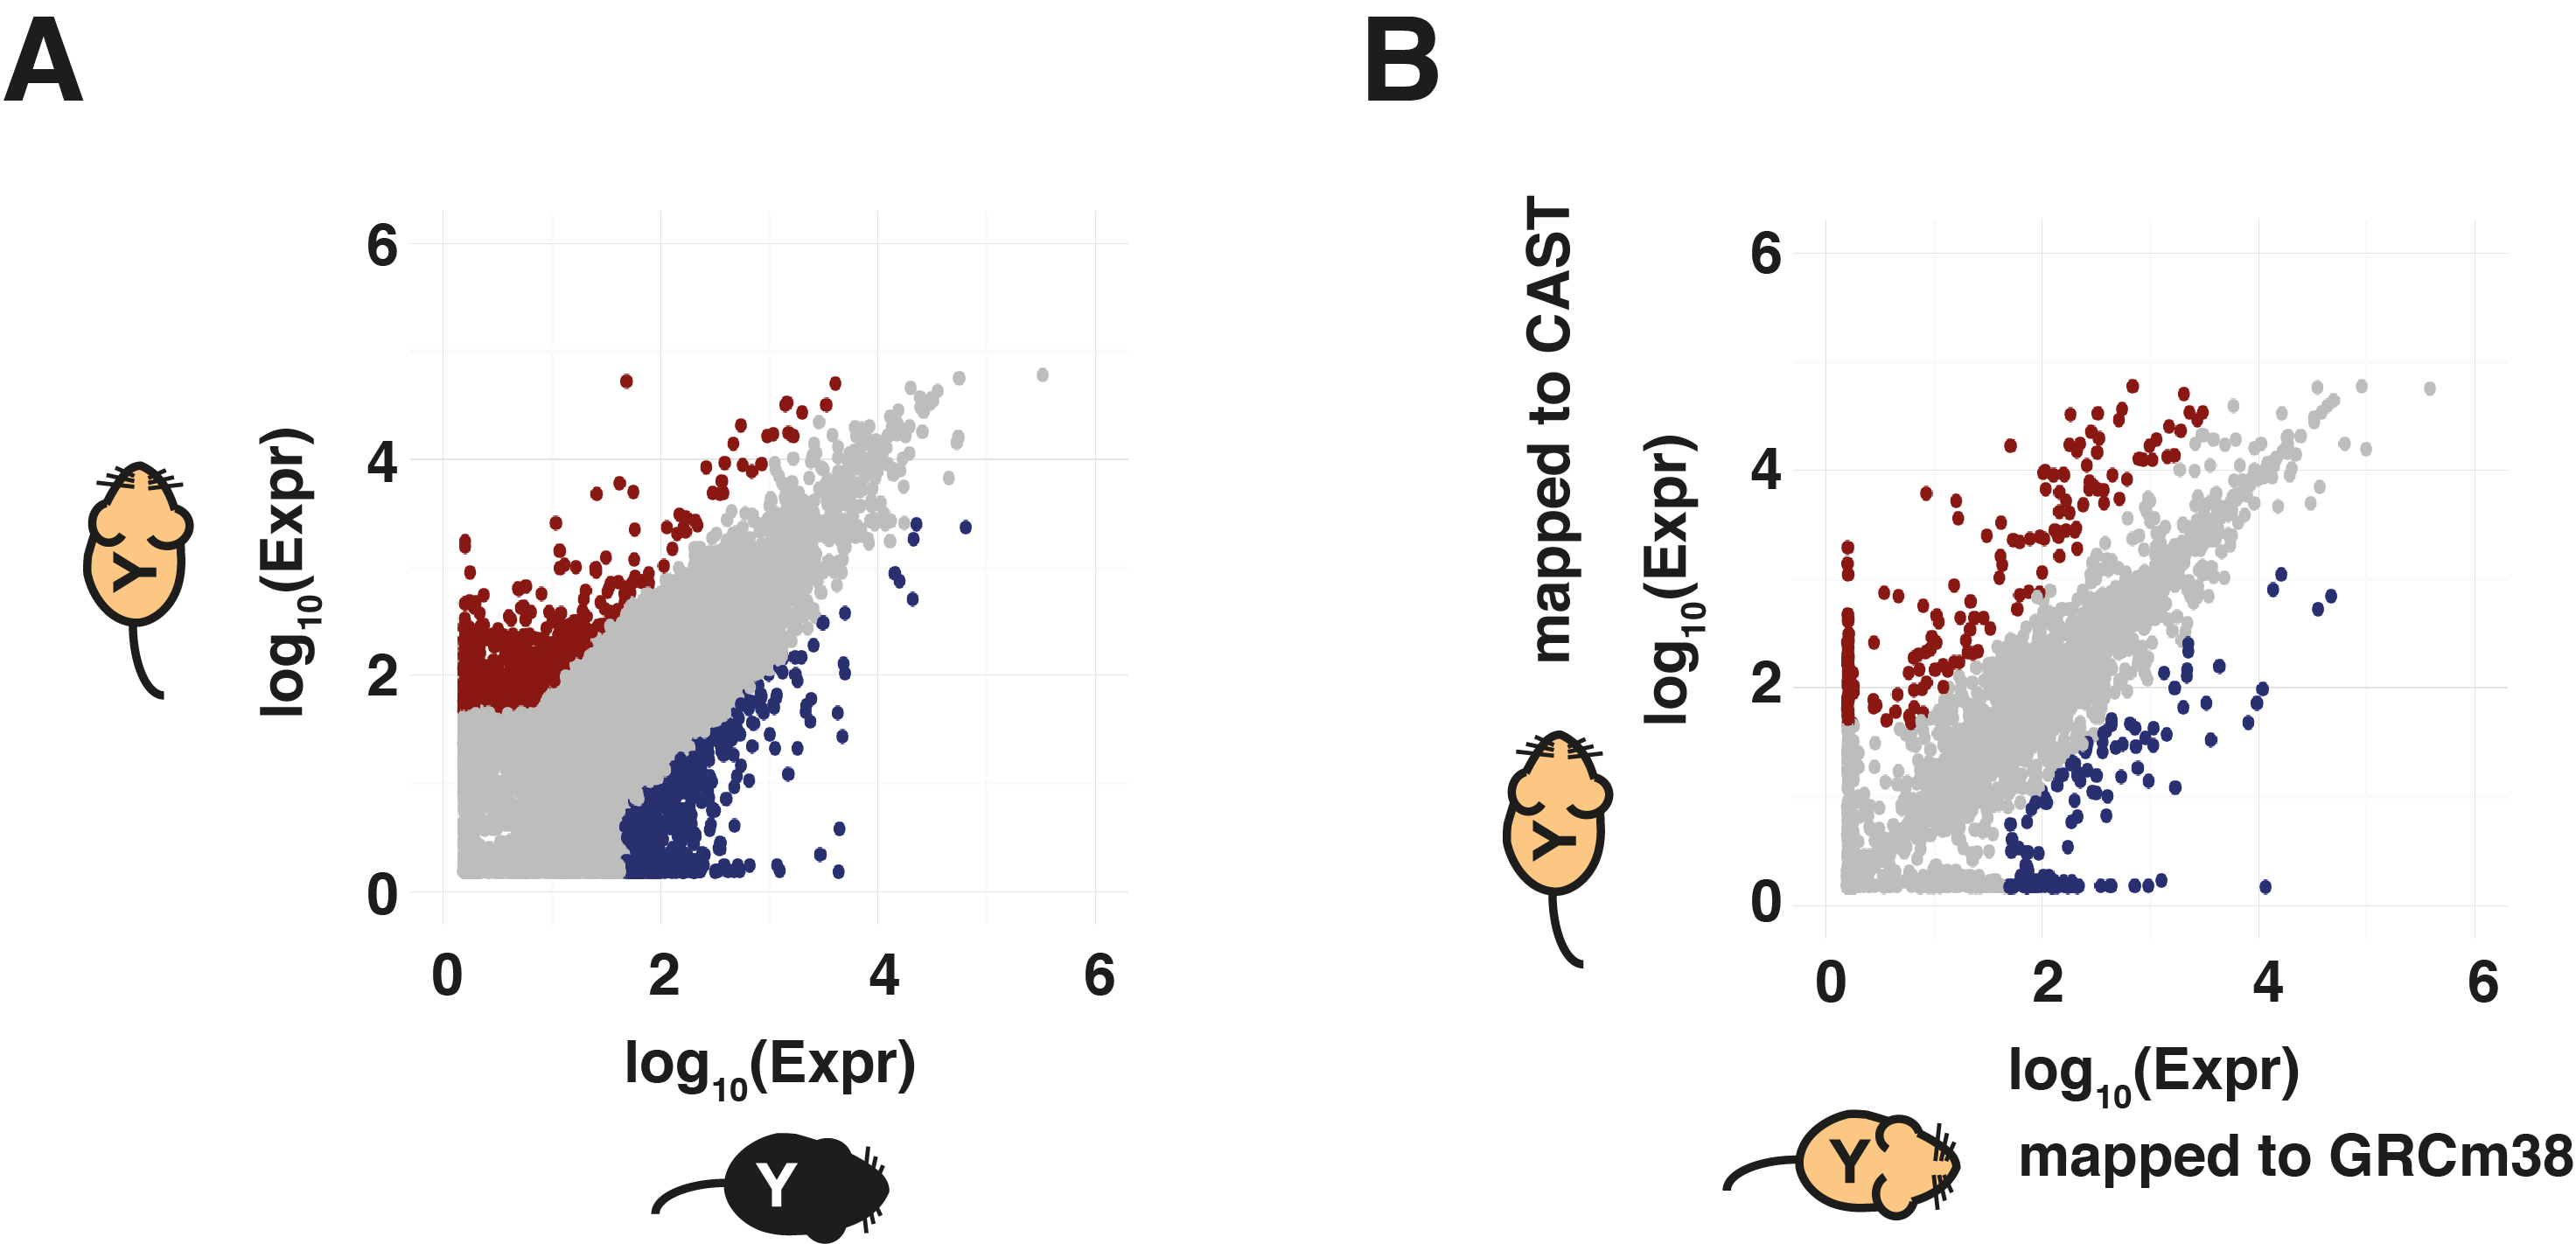
\includegraphics[width=0.8\textwidth]{Fig_7.png}
\caption[Visualization of all isolated CD4$^+$ T cells]{\textbf{Visualization of all isolated CD4$^+$ T cells.}\\
tSNE dimensionality reduction of 1514 CD4$^+$ T cells isolated from young and old mice of two related strains. Cells were labelled based on \textbf{(A)} their activation state, \textbf{(B)} the mouse strain, \textbf{(C)} experimental isolation approach and \textbf{(D)} age.}
\label{fig1:spec_spec_mapping}
\end{figure}

scRNA-seq revealed cell-to-cell transcriptional variability present across these cell populations that is invisible when considering bulk RNA-seq experiments (Fig. 1D, grey panels). Species-specifically transcribed genes are generally more variable on a cell-to-cell basis than are genes expressed in both species, consistent with neutral drift (Fig. S3E).

\newpage


\begin{figure}[!hb]
\centering
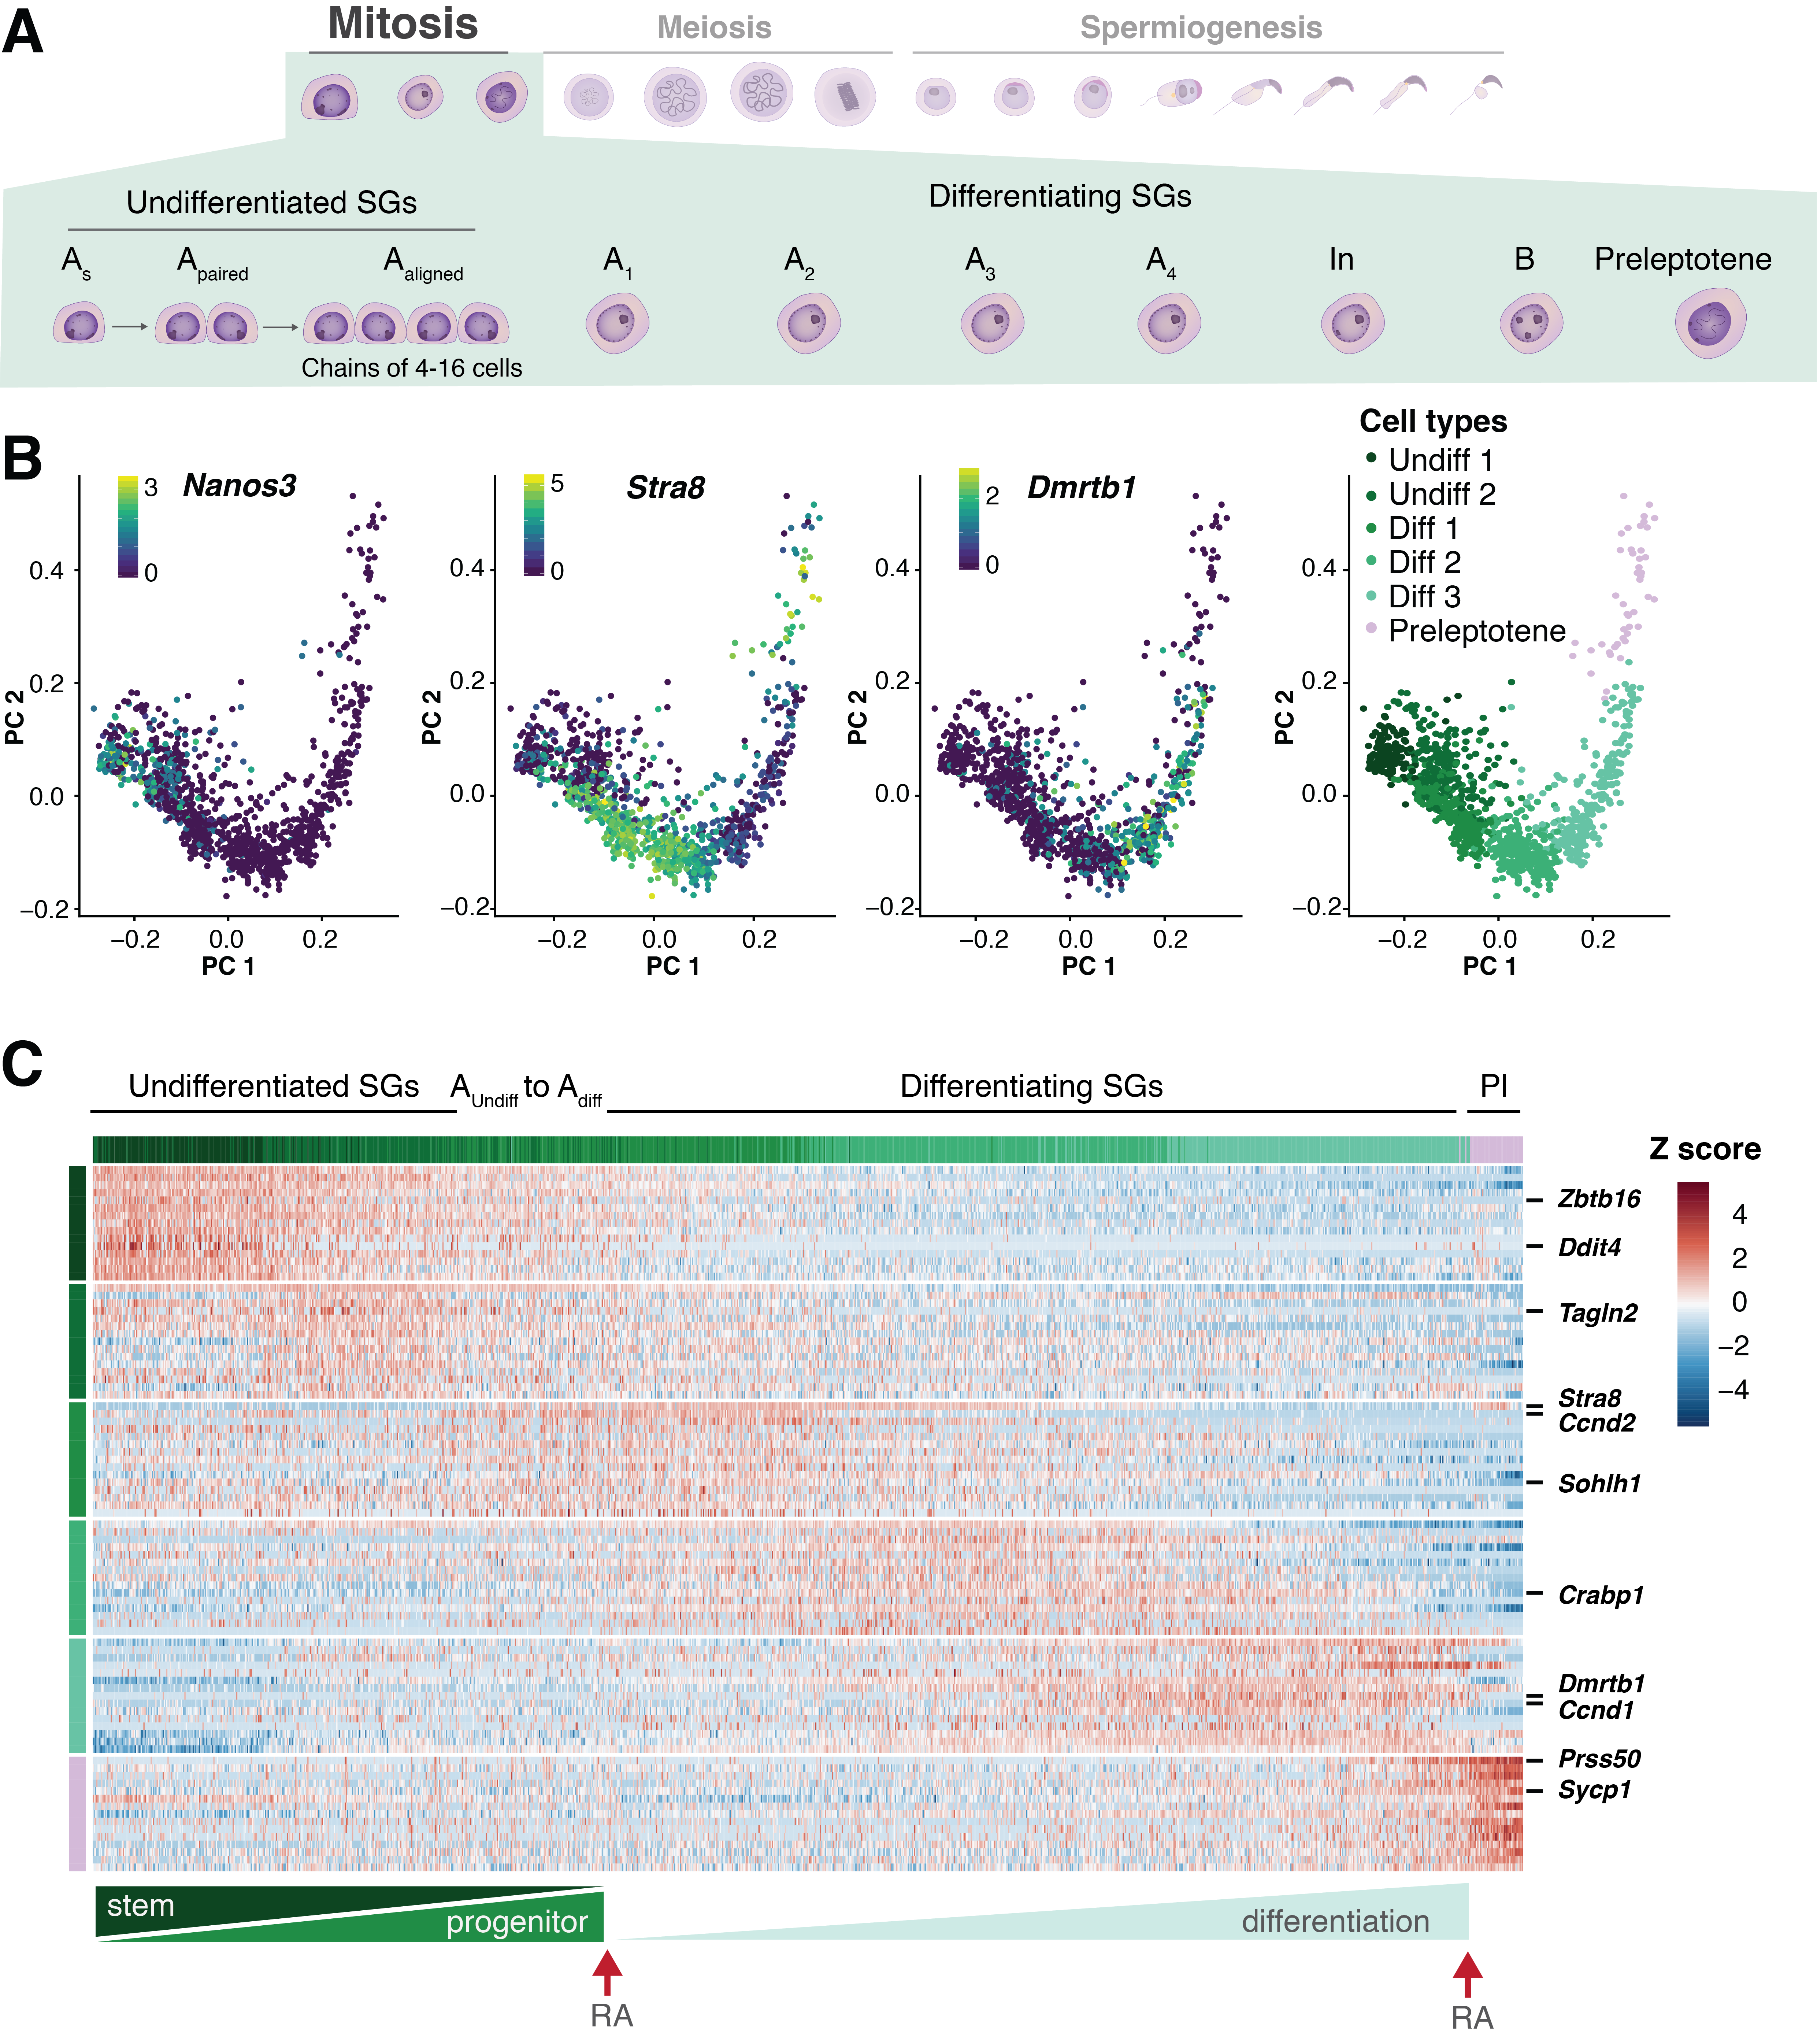
\includegraphics[width=\textwidth]{Fig_6.png}
\caption[Visualization of all isolated CD4$^+$ T cells]{\textbf{Visualization of all isolated CD4$^+$ T cells.}\\
tSNE dimensionality reduction of 1514 CD4$^+$ T cells isolated from young and old mice of two related strains. Cells were labelled based on \textbf{(A)} their activation state, \textbf{(B)} the mouse strain, \textbf{(C)} experimental isolation approach and \textbf{(D)} age.}
\label{fig1:species_specific}
\end{figure}
